\def \imgpath {"./figures/analysis"}
Hadrons \KOs and \LA (\AL) are unstable neutral primary particles that usually decay within the volume of the detector through the weak interaction. Their mean lifetimes are $\sim \cmc{2.7}$ and $\sim \cmc{7.9}$, respectively.\cite{ALICEprimaries} Their dominant decay channels, which are also used for their measurement, are:
\begin{align}
\KOs &\rightarrow \pip \, \pim \\
\LA &\rightarrow \p \, \pim \\
\AL &\rightarrow \pbar \, \pip \, \, .
\end{align}
Because of how these hadrons' decay topologies appear in the detector (an undetectable neutral particle decaying into a V-shaped pair of detectable tracks), they are commonly nicknamed \VOs \footnote{Not to be confused with \VOA and \VOC---the forward calorimeters in ALICE, or \VOM---the related multiplicity estimator using the calorimeters' signal.}. 

\section{Analysed datasets}
TBA
Description of data, collection years, some QA
Monte Carlo
The Monte Carlo data are simulated using a physics event generator (in this measurement, Pythia 8\cite{}) and a model describing the propagation of particles through the detector environment (GEANT\cite{}). 

\section{Identification of \VOs using ALICE}
A centrally developed ALICE algorithm, the ALICE \VO finder, is used to collect suitable \VO candidates from pairs of oppositely charged tracks  with the relevant topology. This typical topology is illustrated in Fig.~\ref{fig:analysis:v0decay.} %More details here and cite
Additional selection criteria (``cuts") are further applied to suppress the background among those candidates. These include:
\begin{itemize}
\item cuts on kinematics of the mother and the daughters,
\item constraints on the topology of the decay,
\item constraints on the reconstruction quality of the daughter tracks,
\item cuts on the specific ionisation energy loss of the daughters, 
\item rejection of contributions from pile-up using ``fast detector" information,
\item rejection of other competing \VO candidates based on their invariant mass.
\end{itemize}
The full list of used cuts is listed in Tab.~\ref{tab:analysis:v0cuts}.

\begin{figure}
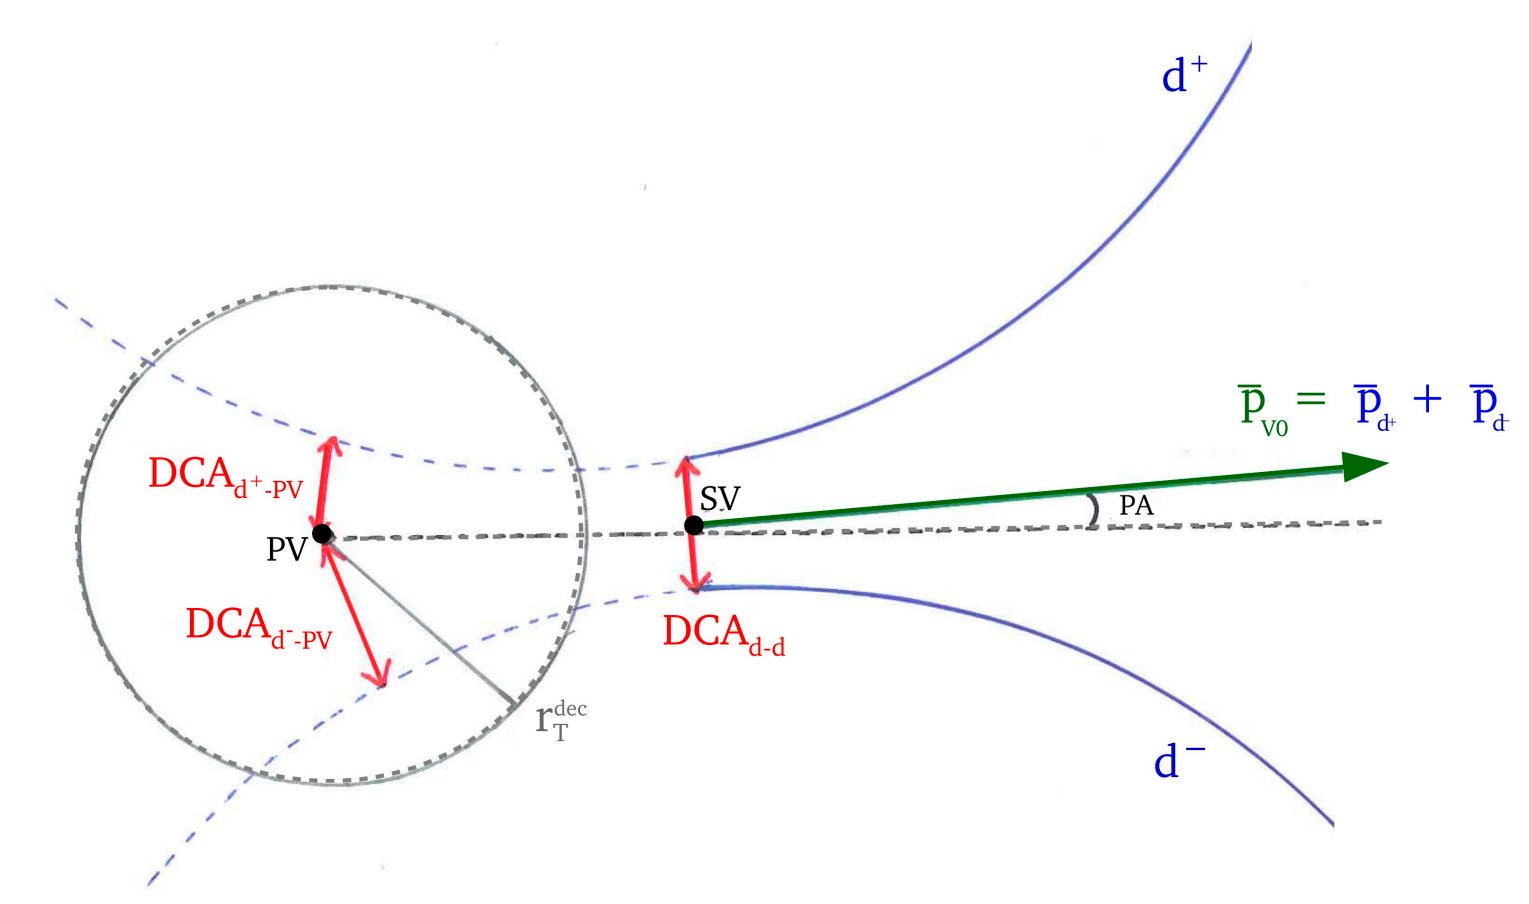
\includegraphics[width=.75\textwidth]{\imgpath/analysis_v0decay.png}
\caption{Typical topology of \VO decay. PV stands for primary vertex, SV for secondary vertex. \citep[p.~102]{tuvathesis}}
\label{fig:analysis:peakfit}
\end{figure}

\begin{table}[h!]
\begin{center}
\caption{Cuts used in the identification of the \Ks , \LA , and \AL particles.}
\label{tab:analysis:v0cuts}
\begin{tabular}{|l|c|}
\hline
 \parbox[b][1.1em]{1em}{}Cut Variable & Cut Value for \Ks (\LA , \AL ) \\ \hline
 
 \multicolumn{2}{l}{\parbox[b][1.2em]{1em}{}Topology} \\ \hline
\parbox[b][1.1em]{1em}{}\VZ pseudorapidity & $-0.8 < \eta < 0.8$ \\
Transverse momentum & $1.0 < \pt < 25.0$ \gev \\
\VZ DCA  & $\mathrm{DCA}^\mathrm{d-d} < 1.0$ \\
Pointing angle & $\cos \mathrm{PA} > 0.97 (0.995)$ \\
Decay radius & $0.5~\mathrm{cm} < R_{xy}$ \\ \hline

\multicolumn{2}{l}{\parbox[b][1.2em]{1em}{}Daughter Tracks Selection} \\ \hline
\parbox[b][1.1em]{1em}{}DCA of daughters to PV &  $\mathrm{DCA}^\mathrm{d-PV}_{xy} > 0.06$ cm \\
TPC PID of daughters & $< 5 \, \sigma$\\
Track pseudorapidity & $-0.8 < \eta < 0.8$ \\
TPC crossed rows & $N_\mathrm{cr} > 70$ \\
TPC crossed rows to findable ratio & $N_\mathrm{cr}/N_\mathrm{f} > 0.8$ \\ \hline

\multicolumn{2}{l}{\parbox[b][1.2em]{1em}{}Candidate Selection} \\ \hline
\parbox[b][1.1em]{1em}{}Proper lifetime (transverse) & $( \, R_{xy} \times m_{(\LA , \AL) } / p_\mathrm{T} < 30$~cm$ \,)$  \\
Competing mass & $ > 4\, \sigma$ \\ \hline


\end{tabular}
\end{center}
\end{table}
% Cuts need more description

\section{Signal extraction}
The \VO signal is separated from the background in distributions of \Minv in several \pt intervals using the so-called sideband method. Assuming the signal peaks around $\dMassVO=\Minv-\MVO=0$ and approximating the background in this region as linear, the subsequent procedure is followed:
\begin{enumerate}
\item the sideband regions are defined. The \Minv spectra are fitted in the $-0.03<\Minv<\gevcc{-0.03}$ interval using a \Chisq-fit with the distribution
\begin{align}
f = [0] + [1]\cdot\Minv + [2] \cdot \Gaus (\mu,\sigma_1^2) + [3] \cdot \Gaus (\mu,\sigma_2^2) \, \, ,
\end{align}
where \Gaus is a Gaussian distribution. This is done in all \pt bins and illustrated in Fig.~\ref{fig:analysis:peakfit}.
\item In each \pt bin, parameter $\sigma$ is obtained as the RMS of $[2] \cdot \Gaus (\mu,\sigma_1^2) + [3]\cdot \Gaus (\mu,\sigma_2^2)$. To calculate the RMS, the distribution is sampled $10^5$ times.
\item Variables $\mu_{\VO}$ and $\sigma_{\VO}$ as functions of \pt are interpolated using \Chisq fit and the parametrisations:
\begin{align}
\mu_{\KOs} (\pt) &= \begin{cases}
              [0]+[1]\cdot \pt + [2]\cdot \pt^2 & \text{if } \pt < \gevc{1.6} ,\\
              [3] & \text{if } \pt \geq \gevc{1.6} ,
          \end{cases} \\
\mu_{\LA,\AL} (\pt) &= \begin{cases}
              [0]+[1]\cdot \pt + [2]\cdot \pt^2 & \text{if } \pt < \gevc{1.9} ,\\
              [3] + [4]\cdot \pt & \text{if } \pt \geq \gevc{1.9} ,
          \end{cases} \\
\sigma_{\VO} (\pt) &= [0] + [1] \cdot \pt + \dfrac{[2]}{\pt} \, \, .
\end{align}
The fitted parametrisations can be seen in Fig.~\ref{fig:analysis:sigex}.
\item In each \pt bin, we define the signal region \textbf{N} as $(\mu_{\VO} - 6\sigma_{\VO};\mu_{\VO} + 6\sigma_{\VO})$ and the sidebands \textbf{A} and \textbf{B} as $(\mu_{\VO} - 12\sigma_{\VO}; \mu_{\VO} - 6\sigma_{\VO})$ and $(\mu_{\VO} + 6\sigma_{\VO};\mu_{\VO} + 12\sigma_{\VO})$. In these regions, we sum together the entries and acquire $N, A, B$. The choice of $6\sigma_{\VO}$ is rather liberal to avoid biases from incorrect determination of the $\mu_{\VO}$ or the imperfect description of the signal peak width $\sigma_{\VO}$
\item Since the background is assumed to be linear, the sum of the two sideband integrals is an accurate estimation of the background in the signal region. Particle yields $Y$ and the corresponding statistical uncertainties $\sigma_Y$ are calculated as
\begin{align}
Y &= N - A - B \\
\sigma_Y &= \sqrt{N+A+B} \, \, ,
\end{align}
due to the fact that the statistical uncertainties in the signal and sideband regions are fully uncorrelated. Illustrations of this step can be seen in Fig.~\ref{fig:analysis:sideband}.
\end{enumerate}

\begin{figure}
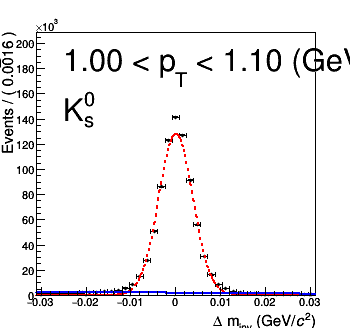
\includegraphics[width=.3\textwidth]{\imgpath/fitK0s.png}
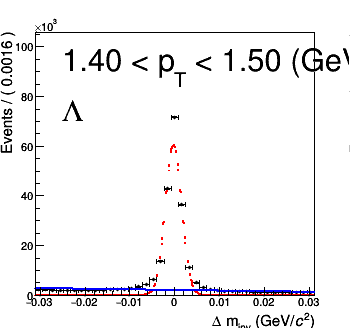
\includegraphics[width=.3\textwidth]{\imgpath/fitL.png}
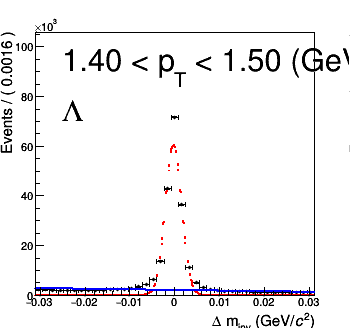
\includegraphics[width=.3\textwidth]{\imgpath/fitL.png}
\caption{Determination of the signal peak mean and width using a fit of the Gaussian distribution for \KOs, \LA, and \AL particles.}
\label{fig:analysis:peakfit}
\end{figure}

\begin{figure}
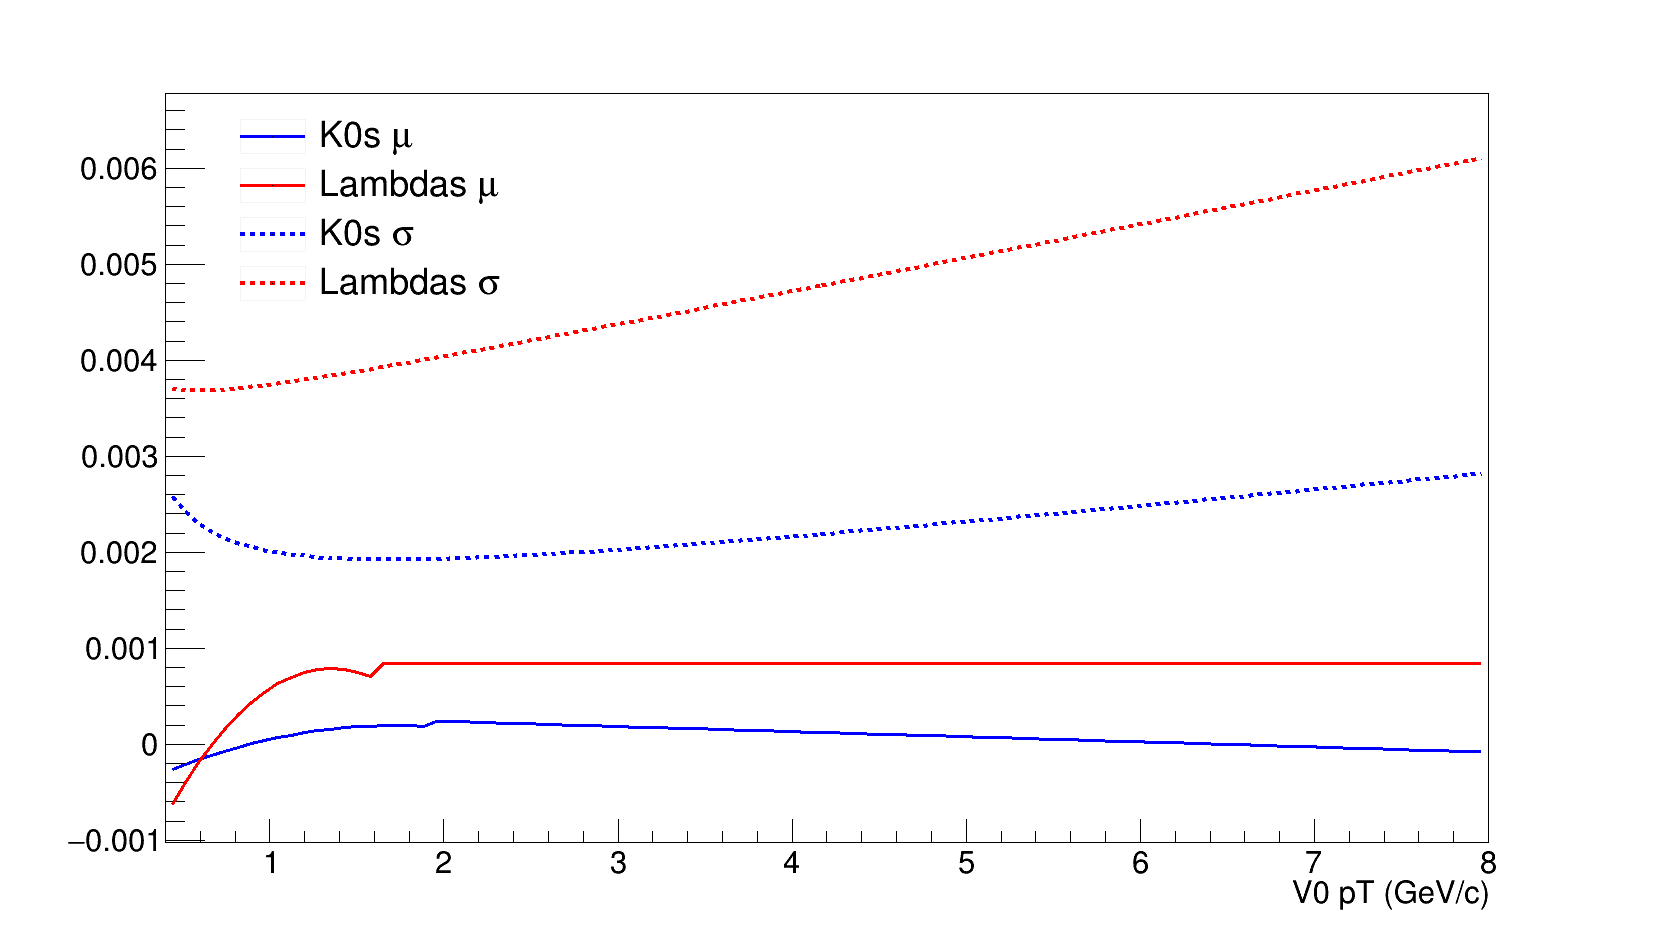
\includegraphics[width=.6\textwidth]{\imgpath/sidebands.png}
\caption{Parametrisation of the signal peak mean and width as a function of \pt.}
\label{fig:analysis:sigex}
\end{figure}


\begin{figure}
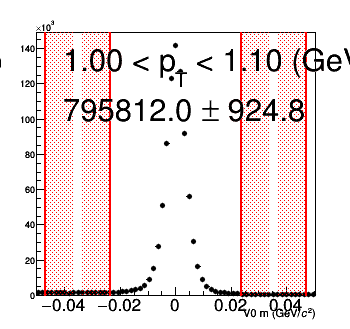
\includegraphics[width=.3\textwidth]{\imgpath/regionK0s.png}
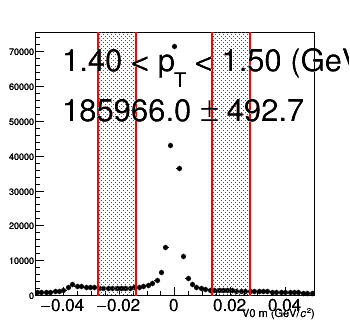
\includegraphics[width=.3\textwidth]{\imgpath/regionL.png}
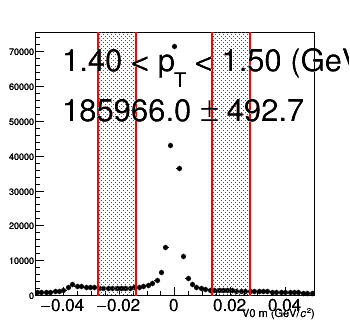
\includegraphics[width=.3\textwidth]{\imgpath/regionL.png}
\caption{Visualisation of the sideband regions, from which the background is estimated, for \KOs, \LA, and \AL particles.}
\label{fig:analysis:peakfit}
\end{figure}


\subsection{Validation using simulations}

The accuracy of the sideband method is tested with ``MC closure"---in MC simulated data, the \pt-spectra acquired blindly from the \VO candidates are compared with \pt-spectra of identified \VO. The ratios can be seen in Fig.~\ref{fig:analysis:sigexclosure} and show a $\sim5 \%$ effect at high-\pt. This is caused by the fact that in ALICE MC simulations, the \VO mass peaks have somewhat longer tails than in data and thus the signal can enter the background regions. This has to be taken into account when defining reconstruction efficiency using MC data.

\subsubsection*{Alternative approach}
Originally, methods involving a likelihood fit and an unbinned likelihood fit of two Gaussian distributions as well as other background descriptions were tested. However, although more sophisticated, these methods proved considerably less precise. This is due to the fact that the signal peaks cannot be accurately described by the two Gaussian distributions, particularly in highly populated \pt bins. That said, they are sufficient to determine the $\sigma_{\VO}$ for above-stated purposes.

\subsubsection*{Mass resolution of secondary \LA and \AL particles}
Approximately 20\% of the \LA yields measured are produced as secondary particles coming from decays of the \XI baryon in most cases -- also called feeddown. Investigations of the simulated data revealed that the invariant mass of these secondaries suffers from a worse resolution (ca.\ 3 times higher $\sigma$). Subsequently, this gives our signal extraction a ca. $75\%$ efficiency for secondaries, and ca. $95\%$ efficiency for inclusive \LA yields at intermediate \pt. This has to be taken into consideration when calculating corrections for the feeddown yields. This effect can be seen in Fig.~\ref{fig:analysis:masssecond}.

\begin{figure}%
\subfloat[][]{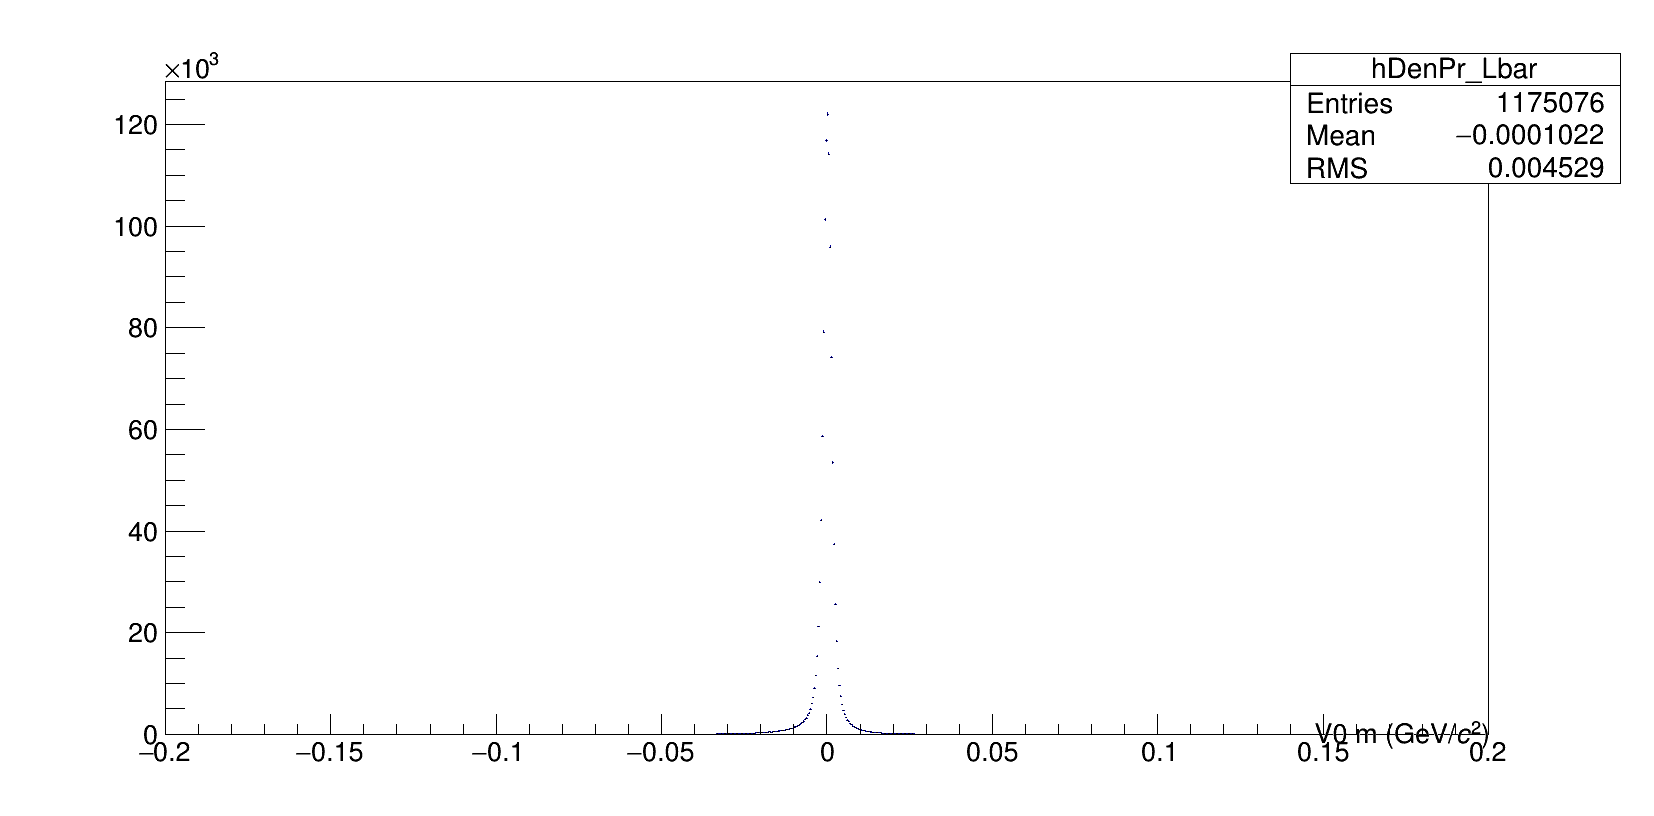
\includegraphics[width=.48\textwidth]{\imgpath/im_primaryPDG.png}}%
\subfloat[][]{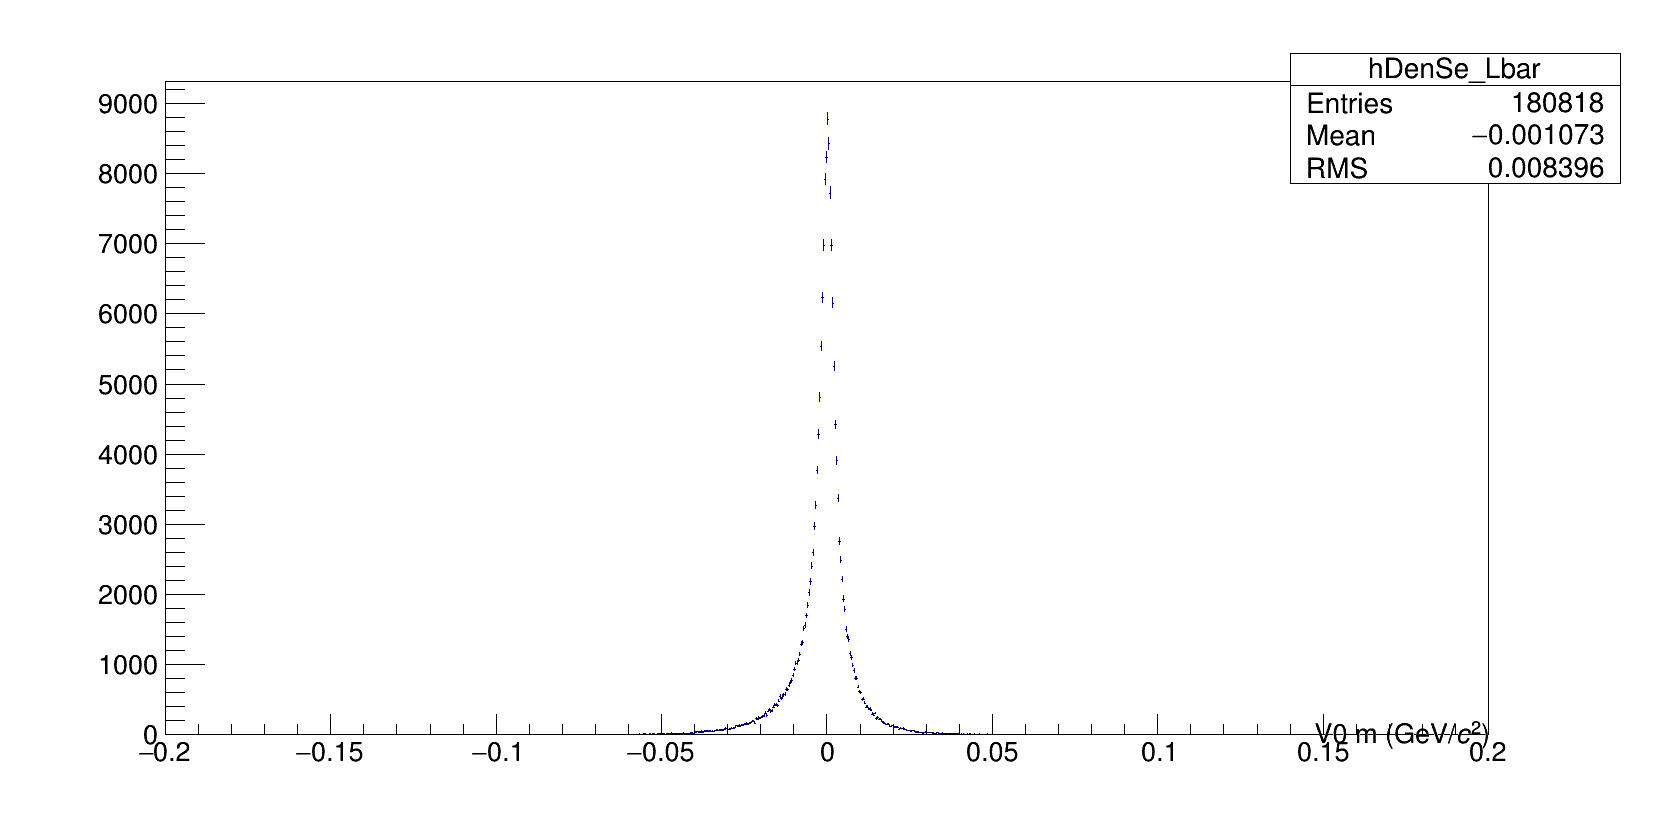
\includegraphics[width=.48\textwidth]{\imgpath/im_secondaryPDG.png}}%
\caption{TBA.}%
\label{fig:analysis:masssecond}%
\end{figure}

\section{Normalisation}

The reconstructed \KOs, \LA, and \AL yields $Y(\eta,\pt)$ are normalised according to

\begin{align}
\frac{\mathrm{d}^2 N^\mathrm{raw}}{\mathrm{d}y \mathrm{d}\pt} = \frac{1}{N_\mathrm{ev}} \frac{1}{J} \frac{1}{\Delta \eta} \frac{1}{\Delta \pt} Y(\eta,\pt) \quad ,
\end{align}
where $N_\mathrm{ev}$ is the number of selected events, $J$ the Jacobian of the $\eta \rightarrow y$ transformation, and $\Delta \eta$ and $\Delta \pt$ the widths of the pseudorapidity and transverse momentum intervals, respectively.

TBA Jacobian

TBA Event loss correction

\section{Corrections to the reconstructed production}

To acquire results with scientific relevance, the raw yields of \VOs observed with ALICE need to be corrected for geometrical acceptance, detector effects, and, in the case of \LA(\AL), also for secondary contribution.

\subsection{Secondary contribution correction}

Only ca.\ $80\%$ of the measured inclusive \LA and \AL yields are produced directly in the pp collision or near-instantanously in non-weak decays of resonances, as primary particles. The remainder is produced secondarily, as products of weak decays of heavier baryons. The dominant, and the only relevant, reactions are:
\begin{align}
\XI^- &\rightarrow \LA \, \pim \, \, , \\
\XI^0 &\rightarrow \LA \, \pi^0 \, \, ,\\
\XI^+ &\rightarrow \AL \, \pip \, \, ,\\
\overline{\XI}^0 &\rightarrow \AL \, \pi^0 \, \, .
\end{align}

For the \KOs, the secondary production (such as from $\phi$ mesons) is negligible.

The primary \LA yields can be estimated using the following equation,
\begin{align}
\LA^\mathrm{raw}_\mathrm{primary} (\pt^i ) &= \LA^\mathrm{raw}_\mathrm{measured} - \LA^\mathrm{raw}_\mathrm{secondary}  \, \, \\
&= \LA^\mathrm{raw}_\mathrm{measured} - \sum_j F_{ij}^\LA \int_{\pt^j} \odv{N}{\pt} (\XI^-) \quad ,
\end{align}
where $F_{ij}$ is the so-called feeddown matrix giving the probabilities of a produced $\XI^-$ or $\XI^0$ particle in a \pt interval $j$ decaying into reconstructed \LA in a \pt interval $i$, and $\odv{N}{\pt} (\XI^-)$ the measured $\XI^-$ spectra.  This approach assumes that the $\XI^0$ decay contribution is identical to $\XI^-$ and is used because $\XI^0$ baryons are challenging to measure. For the \AL , the equation is analogous but uses $\XI^+$ .

The feeddown matrix is calculated in ALICE MC simulations of MB events,
\begin{align}
F_{ij}^\LA &= 2 \, \cdot \, \frac{N_\mathrm{rec.} (\LA) |_{\pt^\LA = i}^{\pt^{\XI} = j}}{N_\mathrm{gen.} (\XI) |_{\pt^{\XI} = j}} \quad ,
\end{align}
where \XI represent both $\XI^-$ and $\XI^0$. There is an assumption that the probabilities, and thus, the matrix, do not depend on multiplicity of the event. It is taken into account in systematic uncertainties.

An alternative approach is constructing $F_{ij}^\LA$ from charged \XI solely, and then multiplying $\LA^\mathrm{raw}_\mathrm{secondary}$ by two and was used to determine the systematic uncertainty.

As discussed previously, due to the worse mass resolution of secondary \LA, a \Minv cut of $5\sigma_{\VO}$ (determined in the sideband definition procedure). Since a large amount of the secondaries enter the background regions, a negative weight $-1$ has to be applied to achieve the best MC closure validation. Other configurations ($6\sigma_{\VO}$ and $-1$ weight, $4\sigma_{\VO}$ and $0$ weight) were also tested.

The feeddown matrices $F_{ij}^{\LA}$, $F_{ij}^{\AL}$ are displayed in Fig.~\ref{fig:analysis:fdmatrix}.

\begin{figure}%
\subfloat[][]{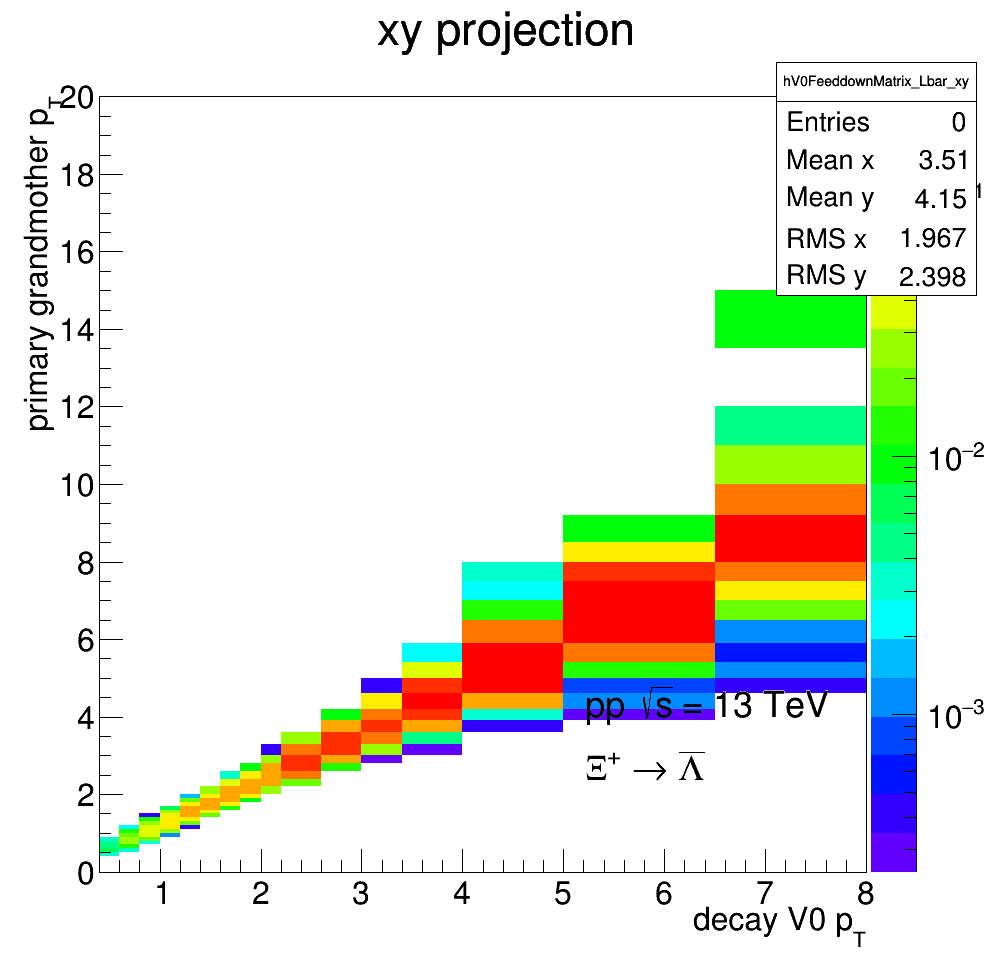
\includegraphics[width=.48\textwidth]{\imgpath/lbar_fdm.png}}%
\subfloat[][]{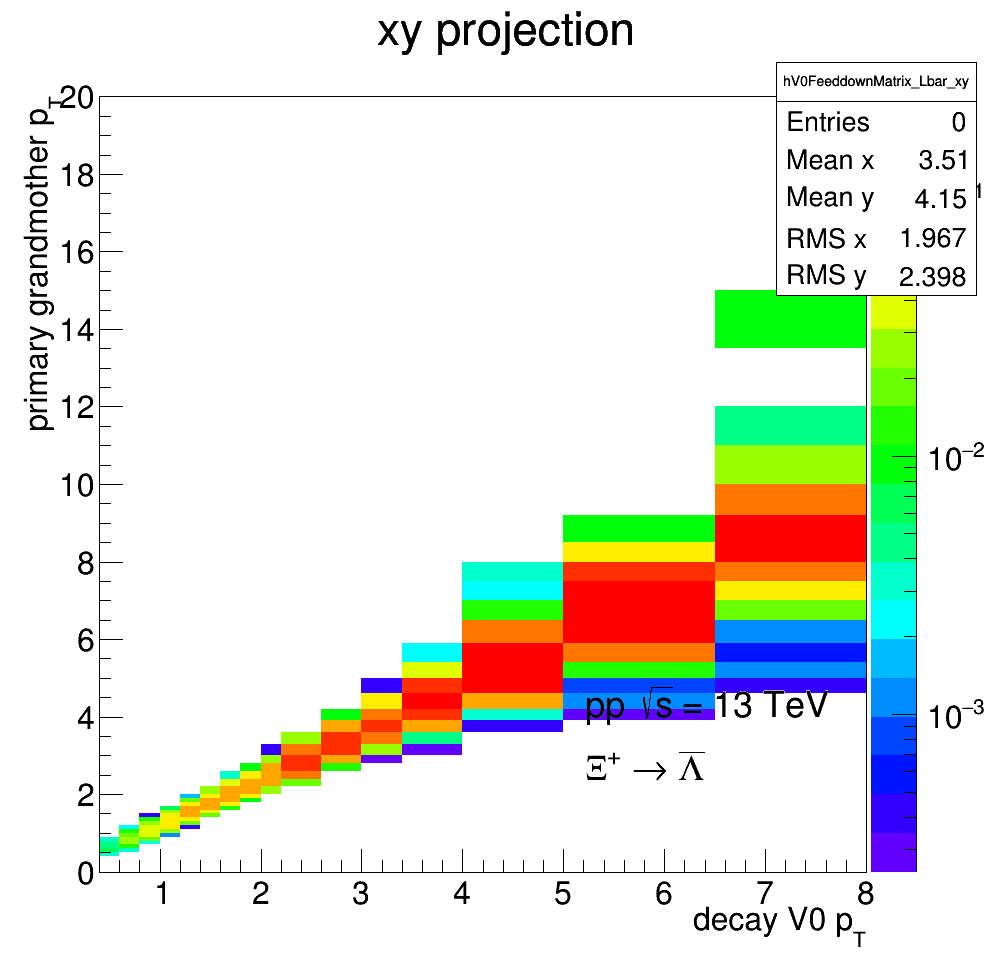
\includegraphics[width=.48\textwidth]{\imgpath/lbar_fdm.png}}%
\caption{Feeddown matrices \textbf{(a)} $F_{ij}^{\LA}$ and \textbf{(b)} $F_{ij}^{\AL}$ from \XI baryons.}%
\label{fig:analysis:fdmatrix}%
\end{figure}

\begin{figure}%
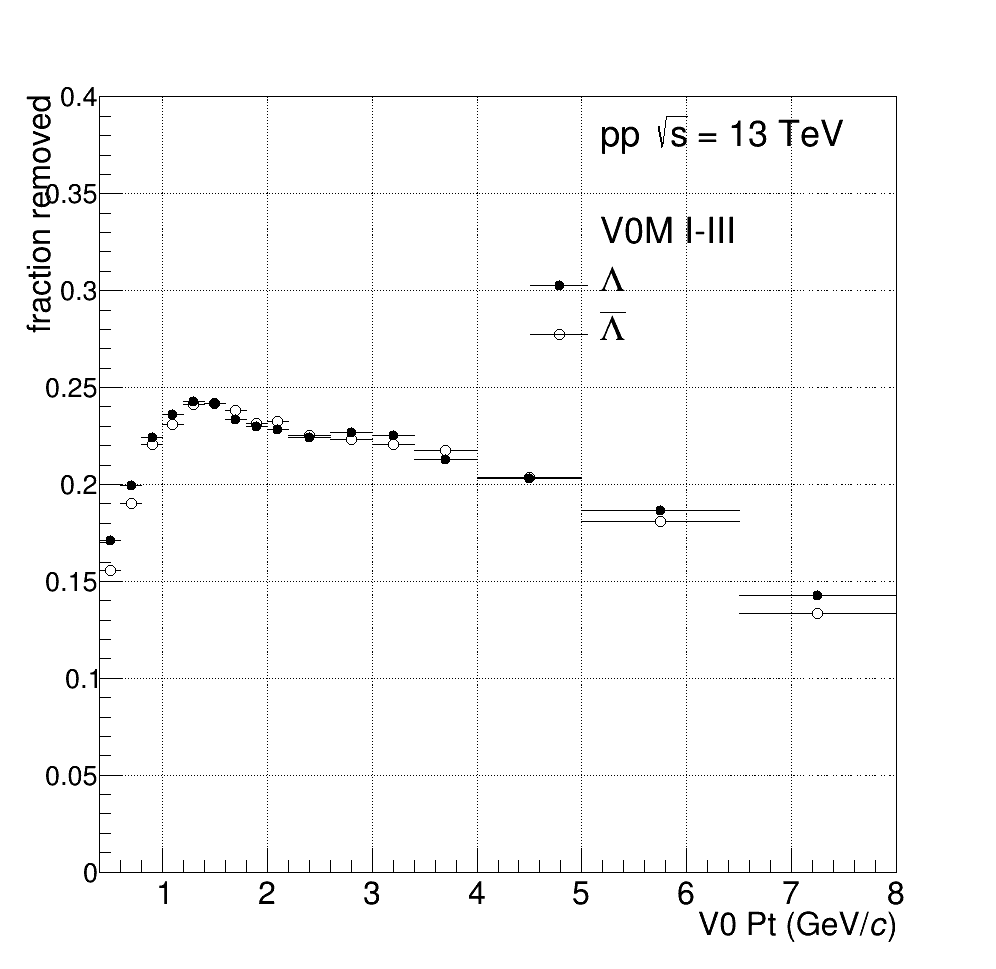
\includegraphics[width=.48\textwidth]{\imgpath/l_fd_hm.png}%
\caption{TBA.}%
\label{fig:analysis:fdfraction}%
\end{figure}

\subsubsection*{\XI spectra}

Fitting. TBA

\subsection{Reconstruction efficiency}

The total reconstruction efficiency, including the acceptance, for \VOs in our events with ALICE can be determined using the Monte Carlo simulated data. It is calculated as
\begin{align}
\epsilon ( \pt ) &= \mathrm{acceptance} \times \epsilon_\mathrm{rec}  \\
&=  \frac{\mathrm{\# \, associated \, reconstructed \, \VOs  }}{\mathrm{\# \, generated \, \VOs \, within \, |\eta|<0.8}}\, \, ,
\end{align}
in events that passed the selection criteria. The association is done by comparing the mother's and daughters' PDG ID as well as the MC generator label. Particles in the numerator have to satisfy all selection cuts. The reconstruction efficiency for \KOs, \LA, and \AL is plotted in Fig.~\ref{fig:analysis:effi}.

As mentioned before, in ALICE simulations, the \Minv resolution worsens with increasing \pt; in high-\pt bins, the simulated \VOs are sometimes reconstructed with higher \Minv than what is considered realistic. This would lead to a lower efficiency as those \VOs can fall out of the signal region, and an overestimation of the total measured spectra. For this reason, a $4\sigma_{\VO}$ cut is required for the \VOs \Minv in the numerator. Alternatively, one could use a cut of $6 \sigma_{\VO}$  and applying a negative weight $-1$ in cases where it is not satisfied. 

The reconstruction efficiency is defined in MB events, assuming the reconstruction in pp collisions does not largely depend on multiplicity, geometrical event classification, or event sub-structure. This assumption is taken into account in systematic uncertainties.

\begin{figure}%
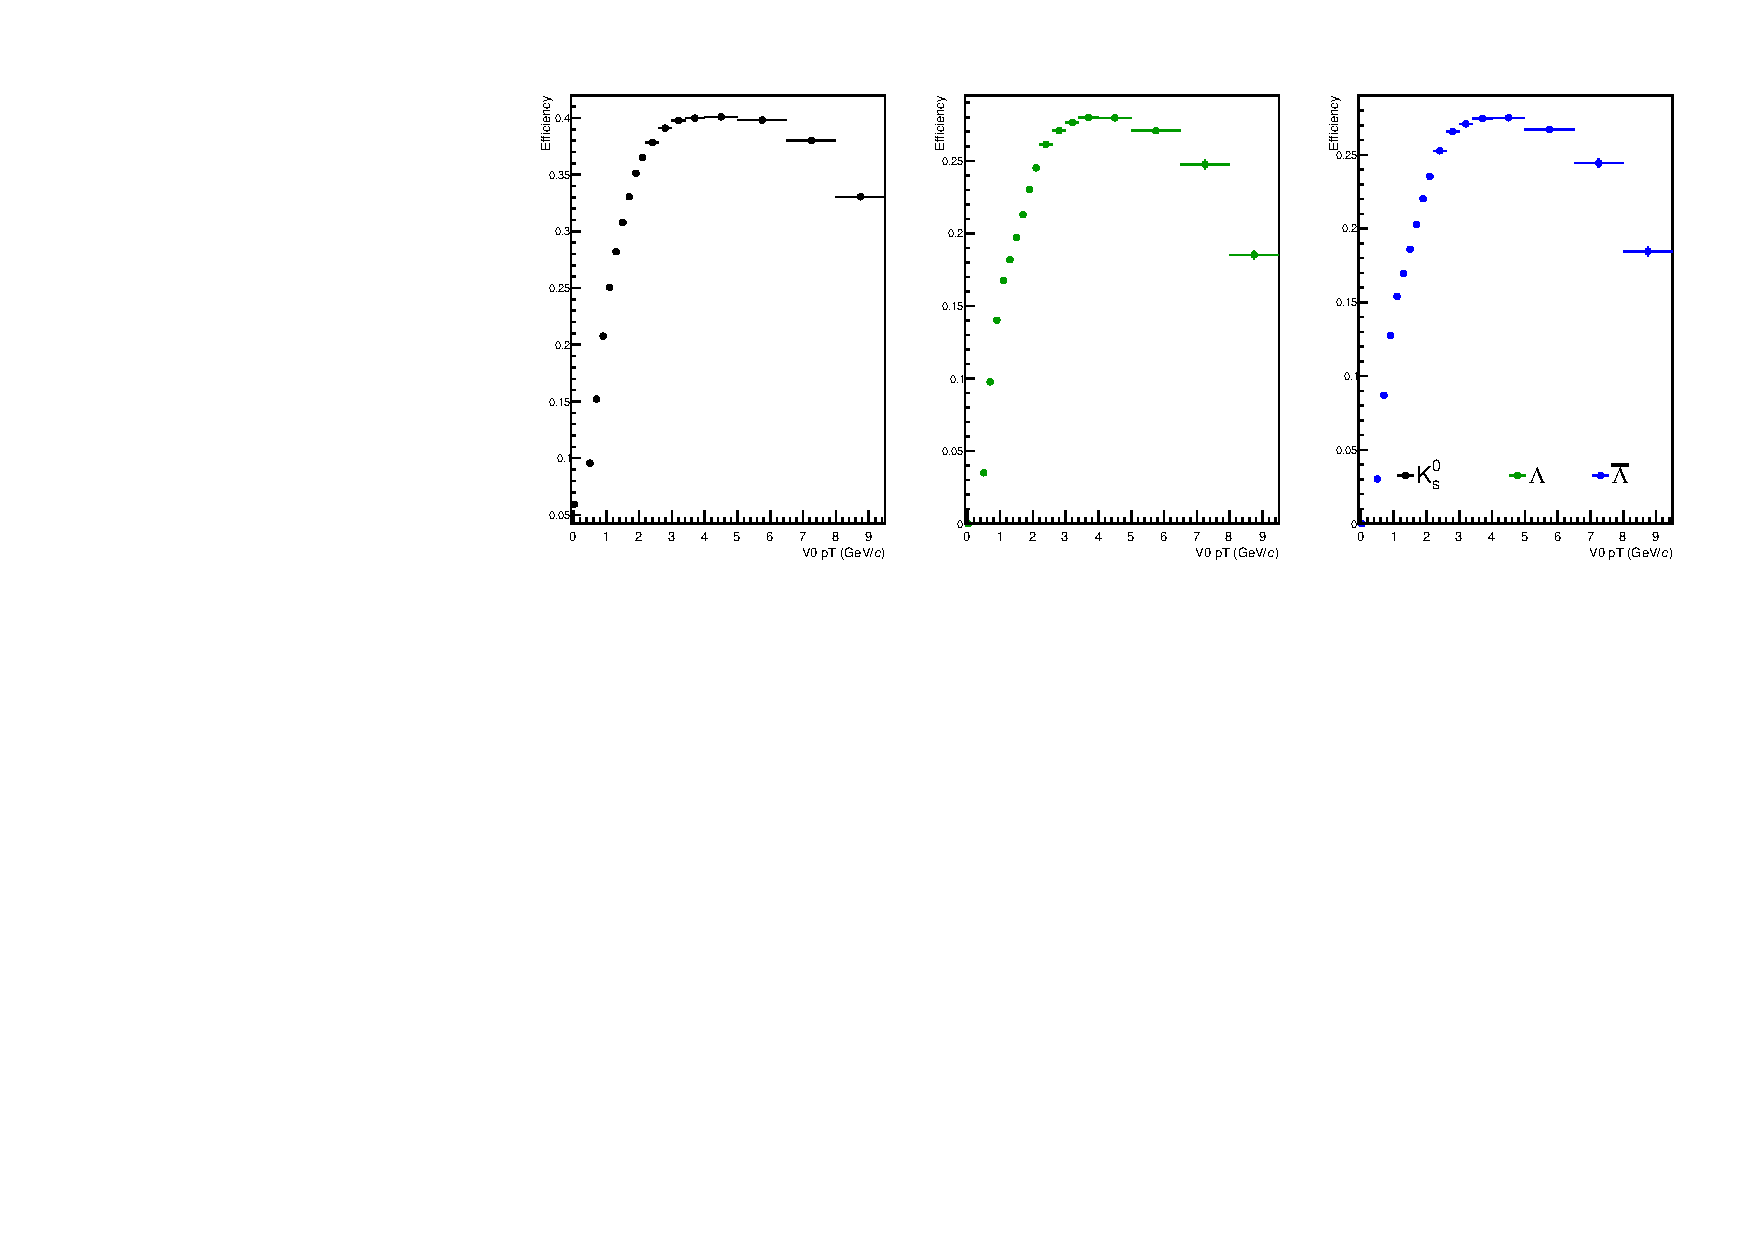
\includegraphics[width=.95\textwidth]{\imgpath/cEffi.pdf}%
\caption{TBA.}%
\label{fig:analysis:effi}%
\end{figure}

\section{Transverse momentum spectra}

Using the corrections on the normalised yields, one acquires the measured transverse momentum spectra, which are comparable with production cross sections and thus theoretical predictions.

\begin{align}
\frac{\mathrm{d}^2 N}{\mathrm{d}y \mathrm{d}\pt} &= \epsilon (\pt) \times \frac{\mathrm{d}^2 N^\mathrm{raw}_\mathrm{primary}}{\mathrm{d}y \mathrm{d}\pt}
\end{align}

\subsection{Comparisons with previously published results}

The acquired results were tested against previously published measurements of \KOs, \LA, and \AL transverse momentum spectra at the ALICE experiment in MB as well as high-multiplicity (\VOM I and \VOM III) events in pp collisions at $\sqrt{s} = 13$~TeV.

\begin{figure}%
%\centering
\subfloat[][]{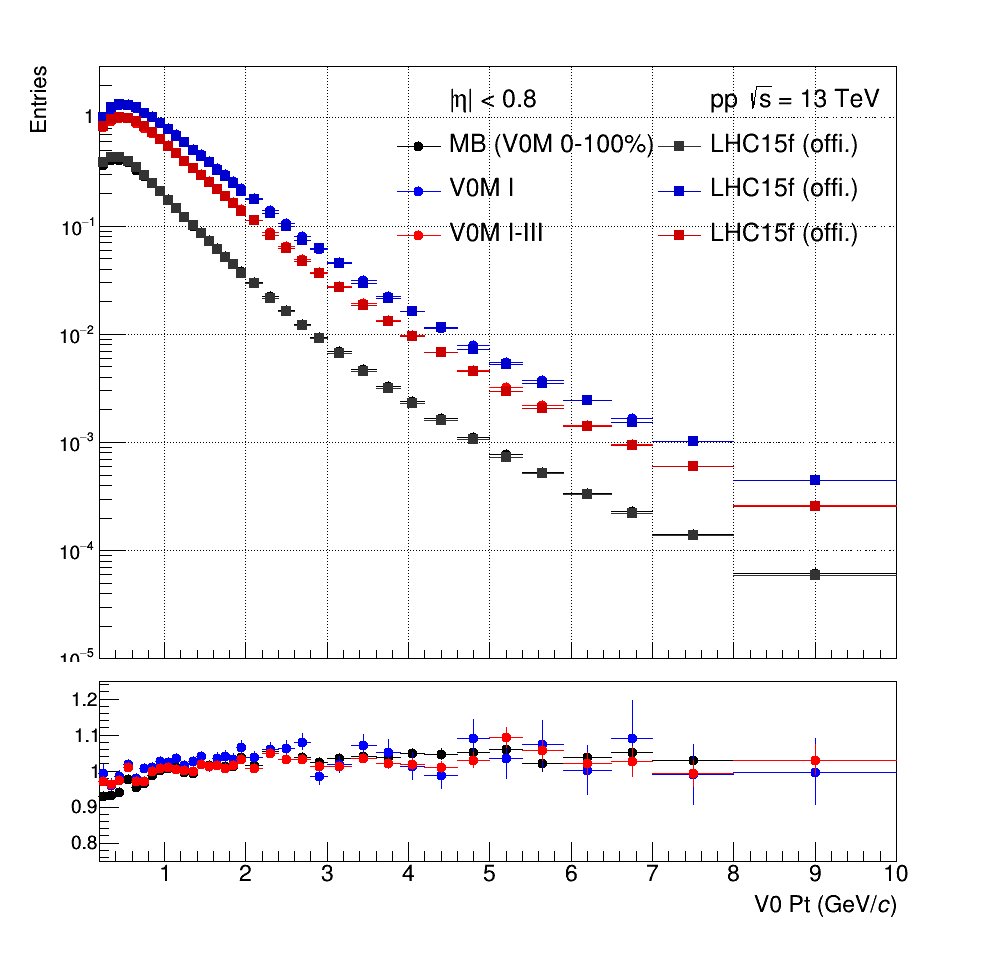
\includegraphics[width=.48\textwidth]{\imgpath/K0toK0_MBandV0M_offi}}%
\subfloat[][]{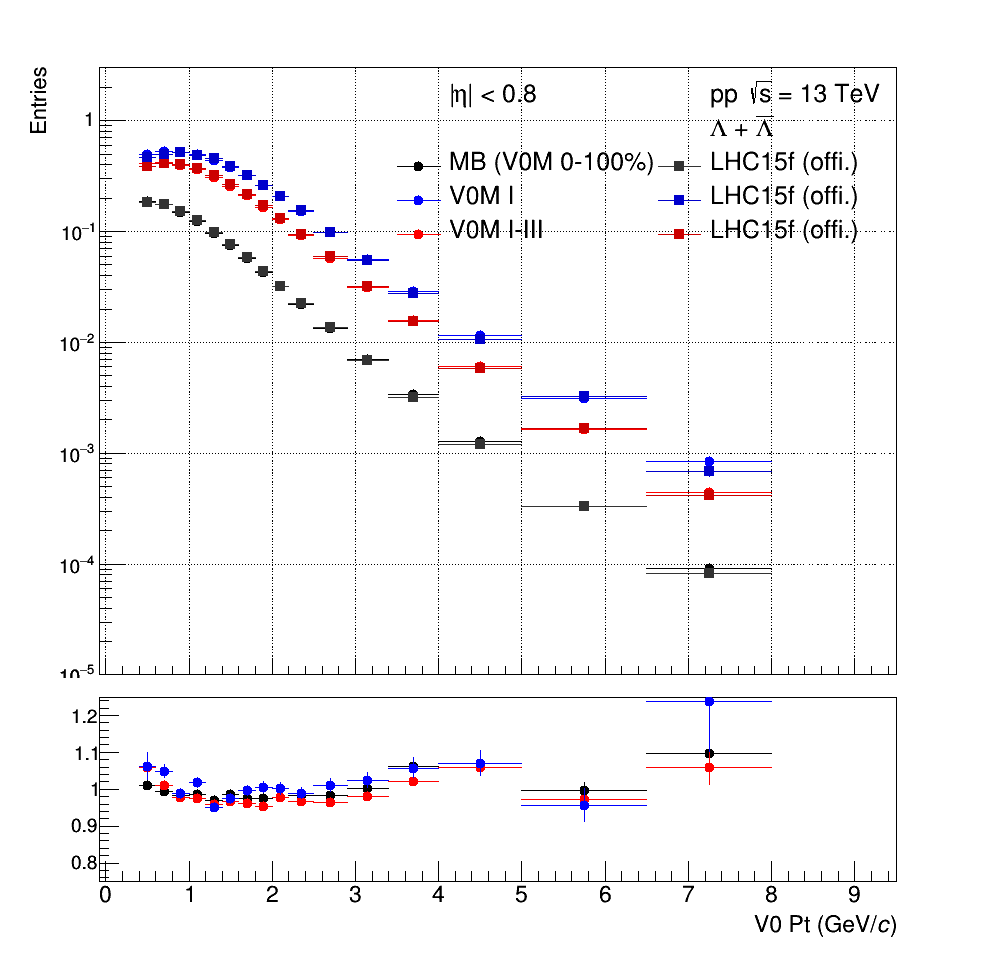
\includegraphics[width=.48\textwidth]{\imgpath/LtoL_MBandV0M_offi.png}}
\caption{Cross-checks of this analysis' \pt spectra of \textbf{(a)} \KOs and \textbf{(b)} \LA + \AL in MB, \VOM I, and \VOM I-III events in pp collisions at against $\sqrt{s} = 13$~TeV results previously published by ALICE.}%
\label{fig:analysis:xcheck}%
\end{figure}

\subsubsection*{\KOs}

The published \KOs results were measured in \spverb|kINT7| events. \cite{} Thus, in order to compare on an equal footing, a trigger efficiency scaling factor $\epsilon_\mathrm{trig} = 0.7448$, taken over from \cite{}, was applied to this analysis.

The comparison of this analysis to the published results can be seen in Fig.~\ref{fig:analysis:xcheck}a. In high-multiplicity events, the spectra are in a good agreement across the entire \pt range (most points lie within $\sim 5\%$ difference). In MB events, there is a difference ($\sim 10 \%$) at the lowest \pt values. This is understood as a loss of signal in events with no reconstructed charged tracks and is usually corrected for. Since the correction plays a role only in MB -- events which are of little interest to this thesis' work -- it is not taken into account.

\subsubsection*{\LA + \AL}

The published \LA + \AL results were measured in same events as this analysis, (\spverb|INEL>0|), therefore, $\epsilon_\mathrm{trig}$ was not applied. \cite{} They are compared to this analysis in Fig.~\ref{fig:analysis:xcheck}b and show a satisfactory agreement (most points lie within $\sim 5\%$ difference).

\section{Systematic uncertainties}

Experimentally measured values always come with uncertainties -- statistical and systematic. Whereas statistical uncertainties are caused by the limited number of measurements and can be decreased by increasing the statistical sample analyzed, systematic uncertainties represent the imprecision or the bias of the experimental methodology itself. Calculation of statistical uncertainties is given directly from frequentist statistics. Definition of systematic uncertanties, however, is not always straightforward -- one cannot simply re-do the measurement with several completely different experimental setups and data analysis techniques. Therefore, a lot of effort needs to go into identifying all possible sources of systematic uncertainties.

In this measurement, the following sources of systematic uncertainty were identified as relevant:
\begin{itemize}
\item \textbf{Variation of selection criteria}\\
In determining the reconstruction efficiency, it is assumed that in ALICE MC simulations, all observables used for the identification of \VOs and for assuring the quality of daughter tracks represent reality. Their inaccurate description, however, results in a bias. This bias is estimated by testing the sensitivity of the final results to varying the selection criteria on these observables.
\item \textbf{Signal extraction method}\\
The biases of the sideband background estimation procedure are tested against increasing and reducing the signal and background regions, by varying the number of $\sigma_{\VO}$. Variations of $5$ and $7 \, \sigma_{\VO}$ were used.
\item \textbf{Multiplicity dependence of $\epsilon ( \pt )$}\\
Studies of the reconstruction efficiency in pp collisions reveal a small, albeit significant dependence on the collision final state. A constant uncertainty of $\sim 2 \%$ is applied on the spectra to account for this.
\item \textbf{Feeddown correction}\\ 
Three sources of uncertainty on the contribution of secondary particles were identified -- variation of the \XI yields, multiplicity dependence of the feeddown matrix, and an alternative method.% First, the \XI yields, from which the feeddown is calculated, are varied within their reported uncertainties. Second, similarily to $\epsilon ( \pt )$, the assumption of no multiplicity dependence of the feeddown matrix is accompanied by a constant uncertainty of $2 \%$ on the secondary yields. Lastly, an alternative method of estimating the feeddown just from charged \XI baryons, and multiplying by a factor of two revealed a systematic uncertainty
\item \textbf{Material budget}\\
This uncertainty reflects that implementing ALICE's material composition in simulations comes with limitations. Previous studies in ALICE \cite{} which varied parameters of the description of the apparatus showed that this effect corresponds to a constant $4\%$ uncertainty on the measured spectra.
\end{itemize}

When testing the default method $A$ against an alternative method $B$, one can implement the deviation of the ratio of their measured values $\Delta = B / A$ from unity as an uncertainty. To ensure that this difference is statistically significant and not just an effect of a limited data sample, the deviation is considered only if it exceeds its own uncertainty, defined as
\begin{align}
\sigma_\Delta = \frac{\sqrt{|\sigma_B^2 - \sigma_A^2|}}{A} \quad ,
\end{align}
where $\sigma_A$ and $\sigma_B$ are the uncertainties of the results from methods $A$ and $B$, respectively.

\subsection{Variation of selection criteria}

To investigate the differences between description of variables in measured data and ALICE simulations, and determine sensible cut variations $\lambda_i$, raw yield loss $F$ was studied. It was measured in MB events and defined as
\begin{align}
F(\lambda) = 1 - \frac{Y(\lambda)}{Y(\lambda_0)} \quad ,
\end{align}
where $Y(\lambda)$ is the raw yield as a function of the cut value $\lambda$ and $\lambda_\mathrm{LOOSEST}$ the loosest variation (corresponding to the highest yield). 

For most observables, the systematic effect can be estimated from alternative methods using $\lambda_\mathrm{LOOSEST}$ and $\lambda_\mathrm{TIGHTEST}$. To ensure the stability and possible non-linearity, less strict $\lambda_\mathrm{LOOSE}$ and $\lambda_\mathrm{TIGHT}$ are also tested. If applicable t is reasonable to choose $\lambda_i$ such that $F(\lambda_i)$ does not exceed approximately $10\%$.

The $F(\lambda)$ for the different selection critera, and with the chosen $\lambda_i$ are shown in Fig.~\ref{fig:analysis:rylK0s}, Fig.~\ref{fig:analysis:rylL}, and Fig.~\ref{fig:analysis:rylAL} for \KOs, \LA, and \AL, respectively. The pile-up rejection cut, which requires ``fast detector" information for at least one daughter is of a binary nature. So, its variation was tested by requiring a different amount of ``fast detector" hits between the two daughters. The selected values of $\lambda_i$ are summarised in Tab.~\ref{tab:analysis:cutvariations}.

\begin{figure}
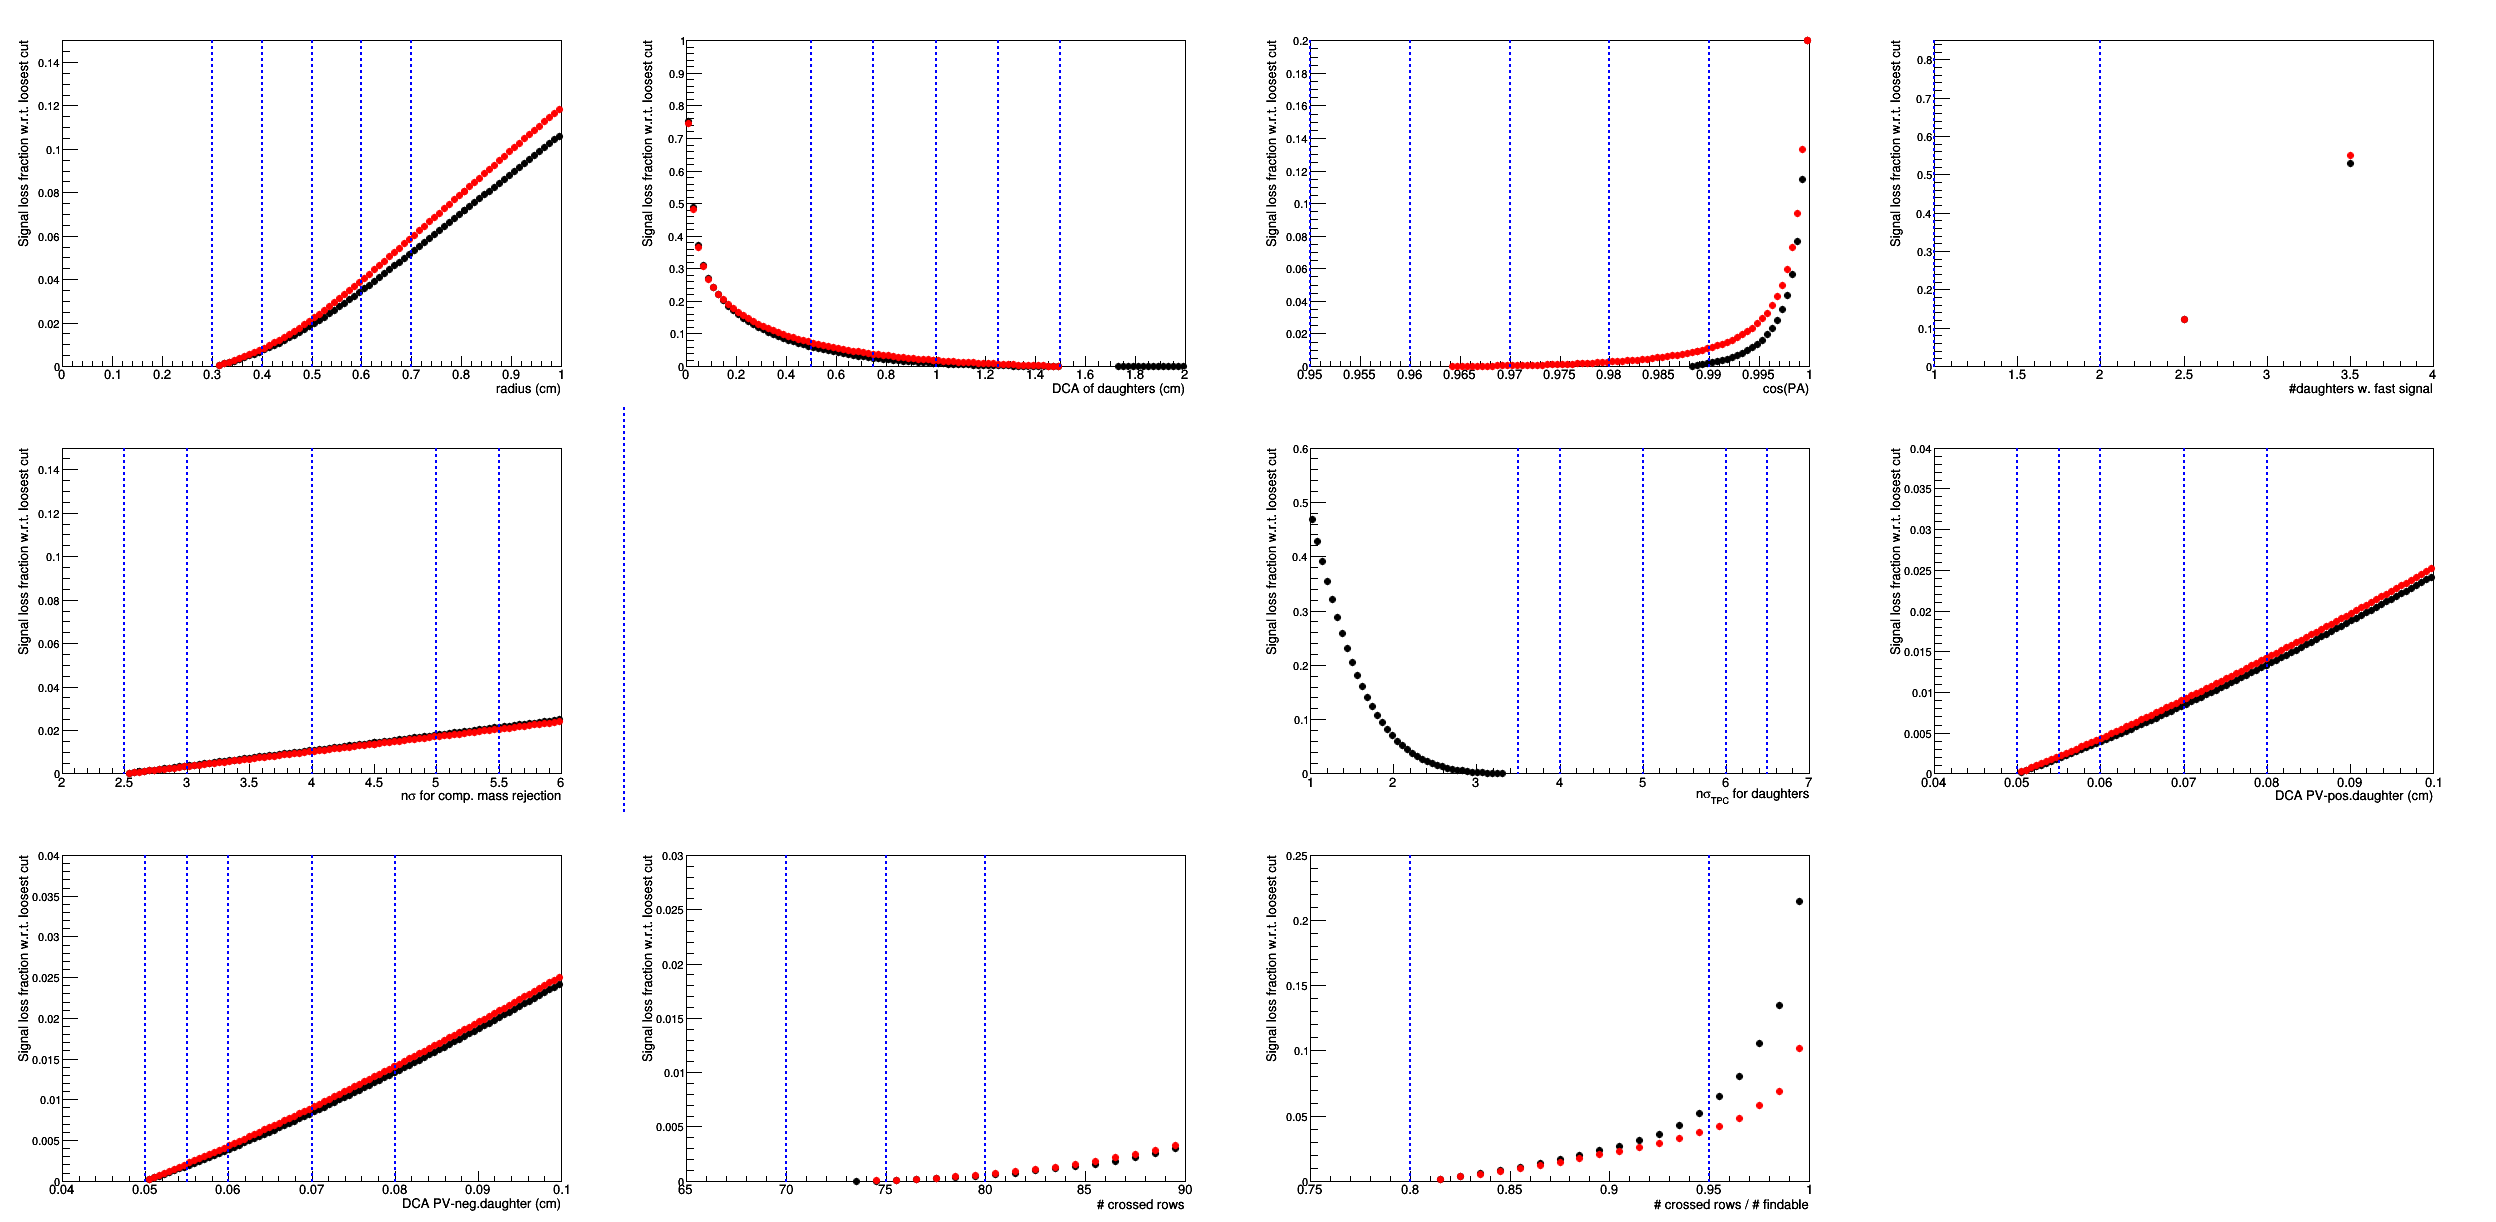
\includegraphics[width=.95\textwidth]{\imgpath/cRYL_K0s.png}
\caption{TBA}
\label{fig:analysis:rylK0s}
\end{figure}

\begin{figure}
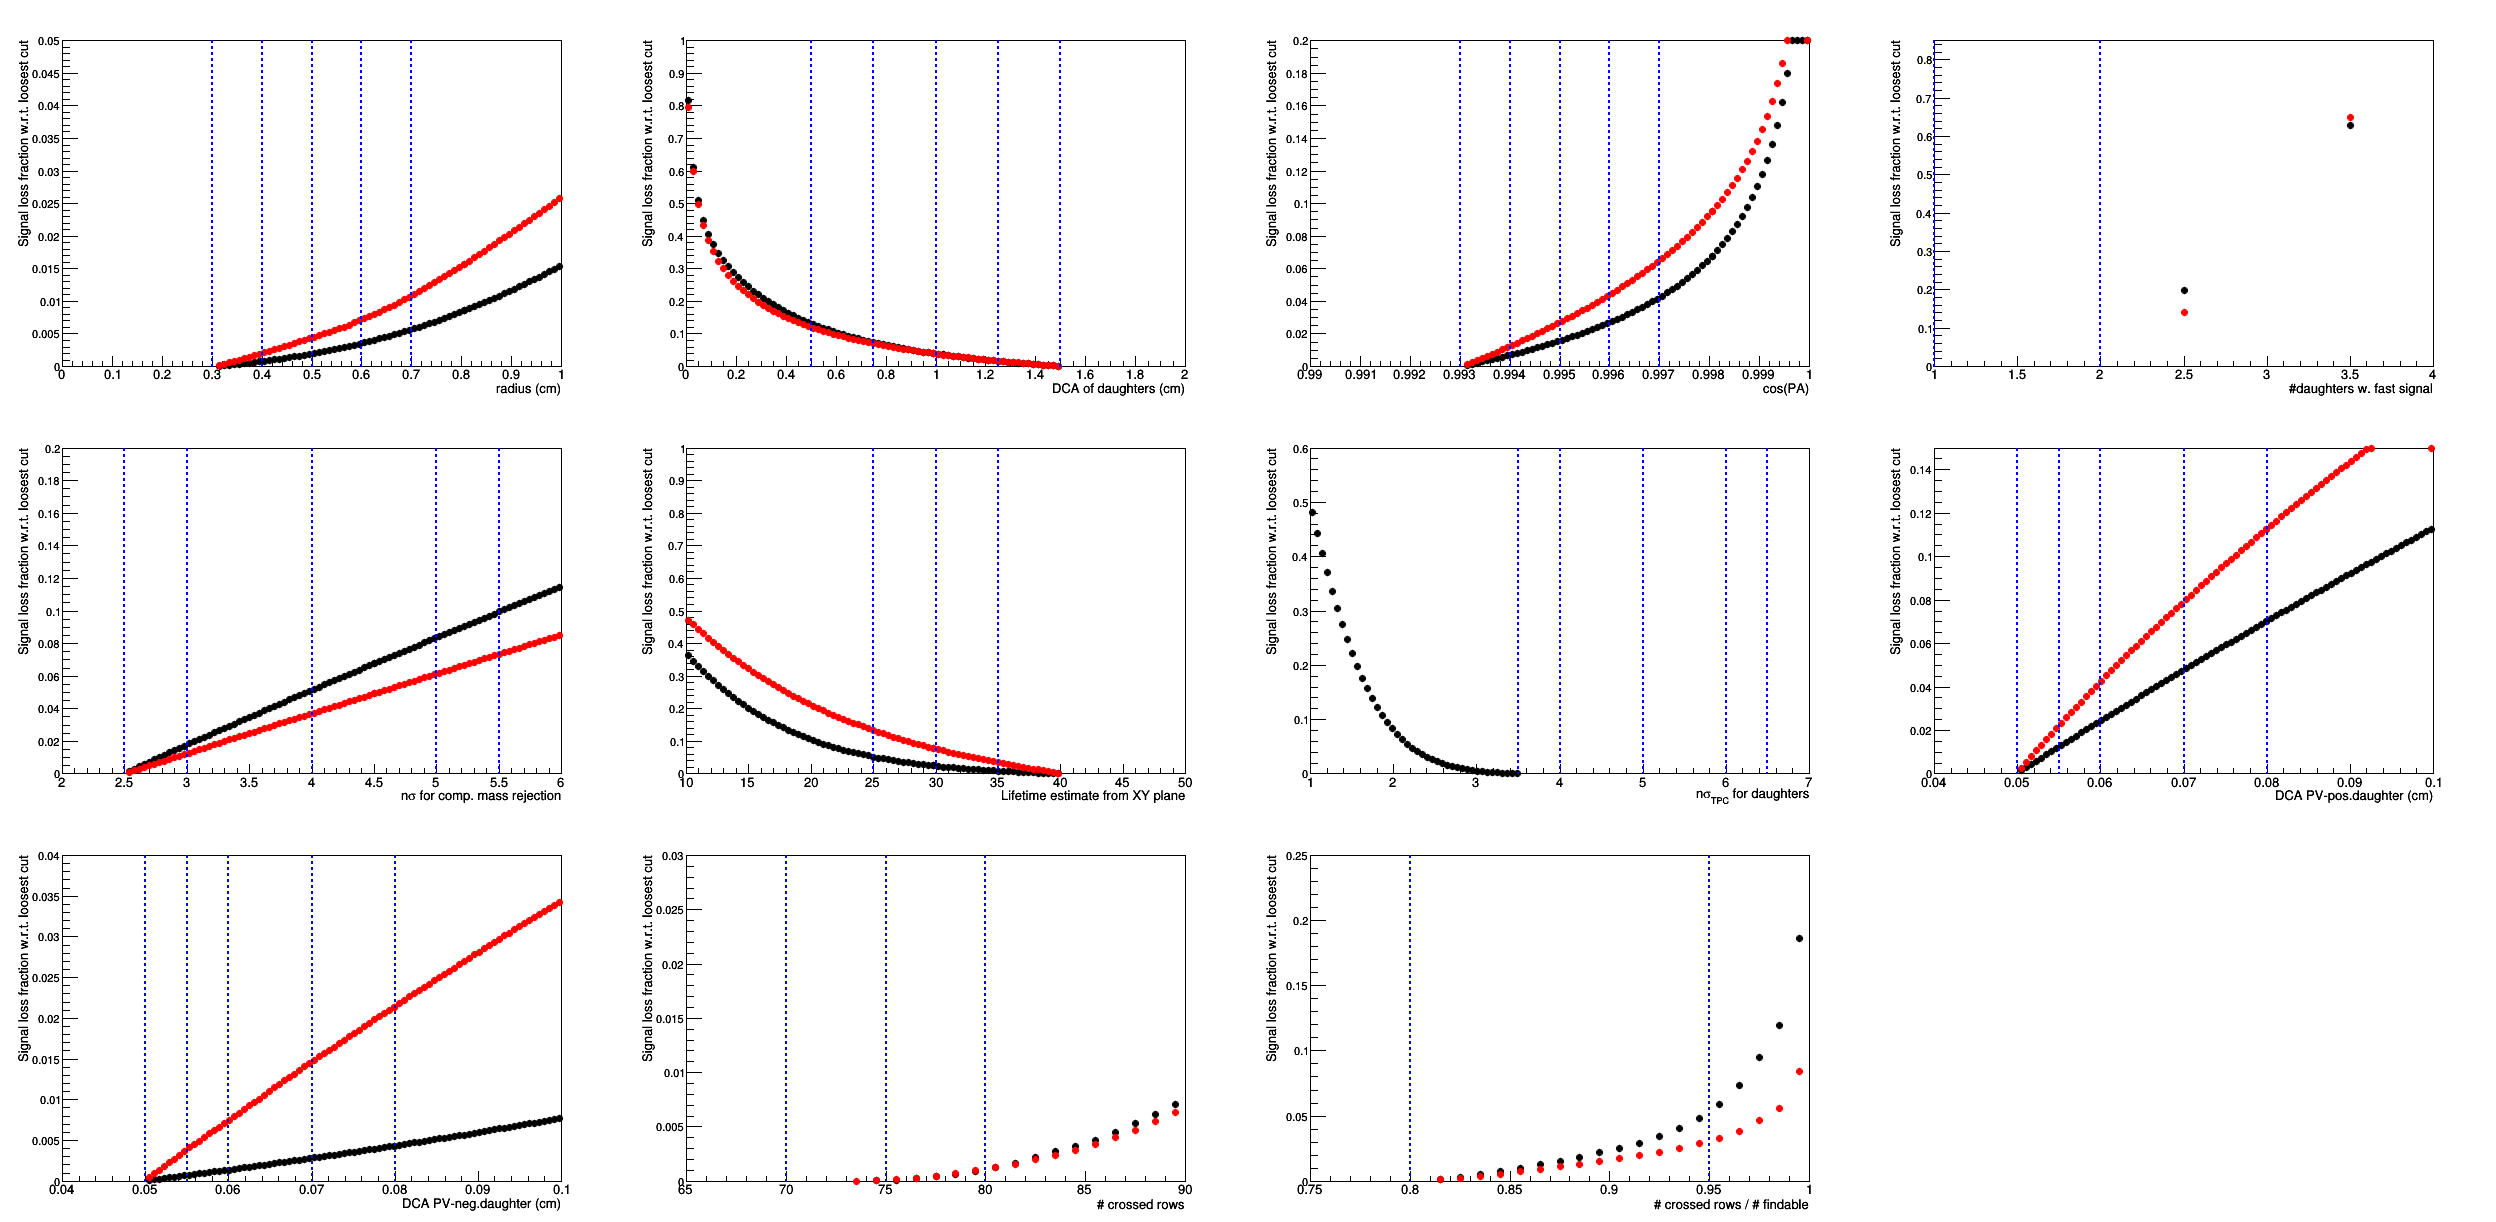
\includegraphics[width=.95\textwidth]{\imgpath/cRYL_L.png}
\caption{TBA}
\label{fig:analysis:rylL}
\end{figure}

\begin{figure}
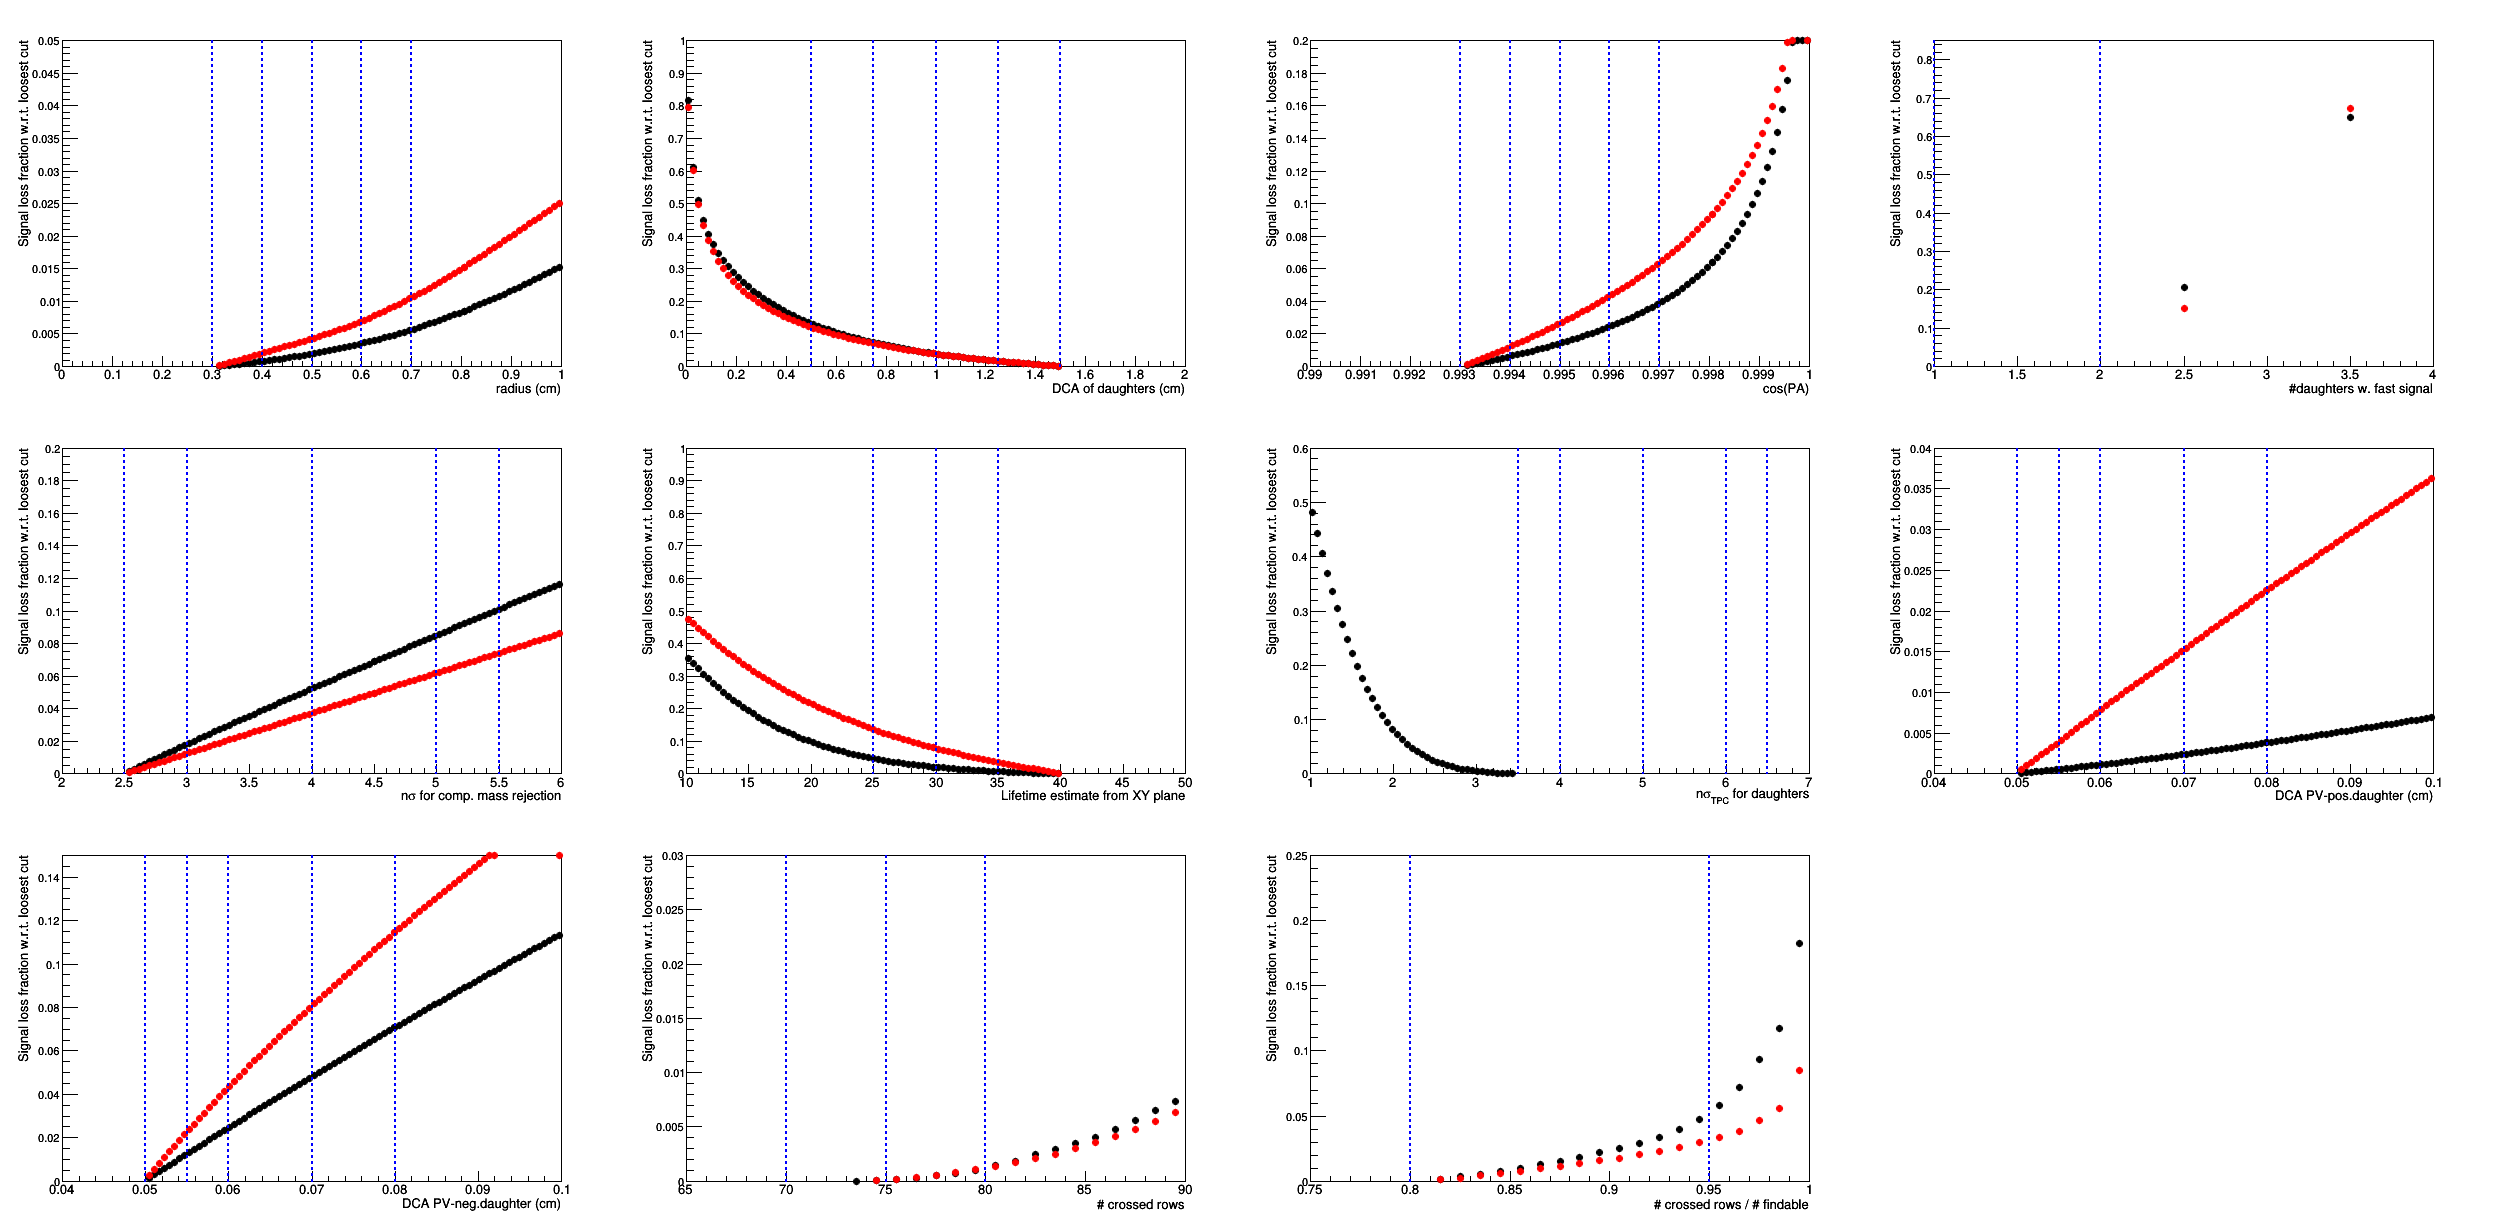
\includegraphics[width=.95\textwidth]{\imgpath/cRYL_Lbar.png}
\caption{TBA}
\label{fig:analysis:rylAL}
\end{figure}

\begin{table}[h!]
\begin{center}
\begin{tabular}{|c|c|c|c|c|c|}
\hline
 \bf Quality & \bf loosest & \bf loose & \bf default & \bf tight & \bf tightest \\ \hline
radius & 0.3 & 0.4 & 0.5 & 0.6 & 0.7 \\ \hline
DCA between daughters & 1.5 & 1.25 & 1.0 & 0.75 & 0.5 \\ \hline
cos PA & 0.95 (0.993) & 0.96 (0.994) & 0.97 (0.995) & 0.98 (0.996) & 0.99 (0.997) \\ \hline
pile-up removal cut & - & - & 1 & 2 & - \\ \hline
comp.\ mass number of $\sigma$ & 2.5 & 3.0 & 4.0 & 5.0 & 5.5 \\ \hline
lifetime & - & (35.0) & (30.0) & (25.0) & - \\ \hline
TPC PID number of $\sigma$ & 6.5 & 6.0 & 5.0 & 4.0 & 3.5 \\ \hline
DCA to PV of pos.\ track & 0.05 & 0.055 & 0.06 & 0.07 & 0.08 \\ \hline
DCA to PV of neg.\ track & 0.05 & 0.055 & 0.06 & 0.07 & 0.08 \\ \hline
TPC crossed rows & - & - & 70 & 75 & 80 \\ \hline
TPC find.\ ratio & - & - & 0.8 & 0.95 & - \\ \hline
\end{tabular}
\end{center}
\caption{Cut variation parameters for the \KOs (\LA and \AL).}
\label{tab:analysis:cutvariations}
\end{table}

\subsection{Feeddown correction}

As mention before, first, the \XI spectra, from which the feeddown is calculated, are varied within their reported uncertainties. In both variations, the yields are then extracted using a fit.  Second, similarily to $\epsilon ( \pt )$, the assumption of no multiplicity dependence of the feeddown matrix is accompanied by a constant uncertainty of $2 \%$ on the secondary yields (corresponding to ca.\ $0.6\%$ uncertainty on the primary yields). %WRONG ACTUALLY

Lastly, an alternative method of estimating the feeddown just from charged \XI baryons, and multiplying by a factor of two, was also tested and contributes a systematic uncertainty. It is considered significant and applied when $|\Delta - 1| > \sigma_\Delta$. The difference between the two methods can be seen in Fig.~\ref{fig:analysis:fdmethod}. It should be noted that whilst the secondary yields suffer from a rather large systematic uncertainty, the effect on the primary spectra is significantly smaller, as the uncertainties enter as $\frac{1-B}{1-A}$ and the secondary yields do not exceed $\sim 30\%$.

\begin{figure}
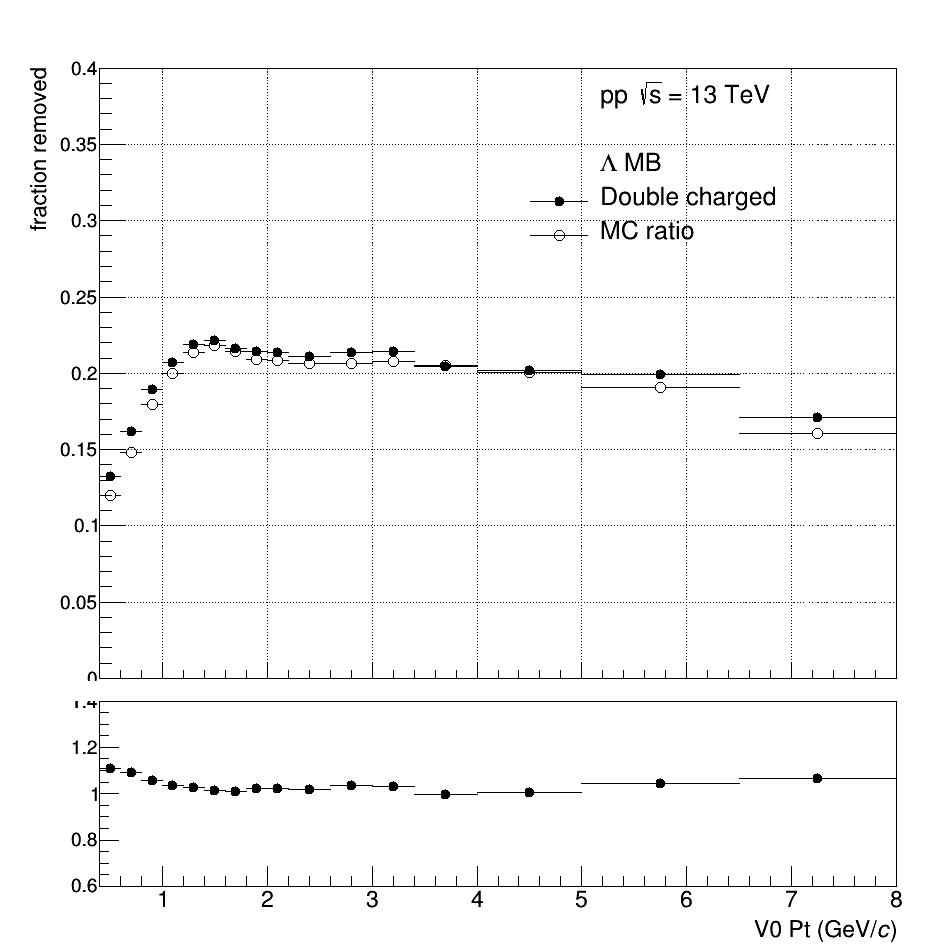
\includegraphics[width=.65\textwidth]{\imgpath/L_fd_mb.png}
\caption{TBA}
\label{fig:analysis:fdmethod}
\end{figure}


